% Systemmodell
\section{Systemmodell}
Die Anwendung st nach dem prinzip des MVC-Entwurfmusters aufgebaut. Das folgende Diagramm zeigt, wie die Software gegliedert ist.
\begin{figure}
    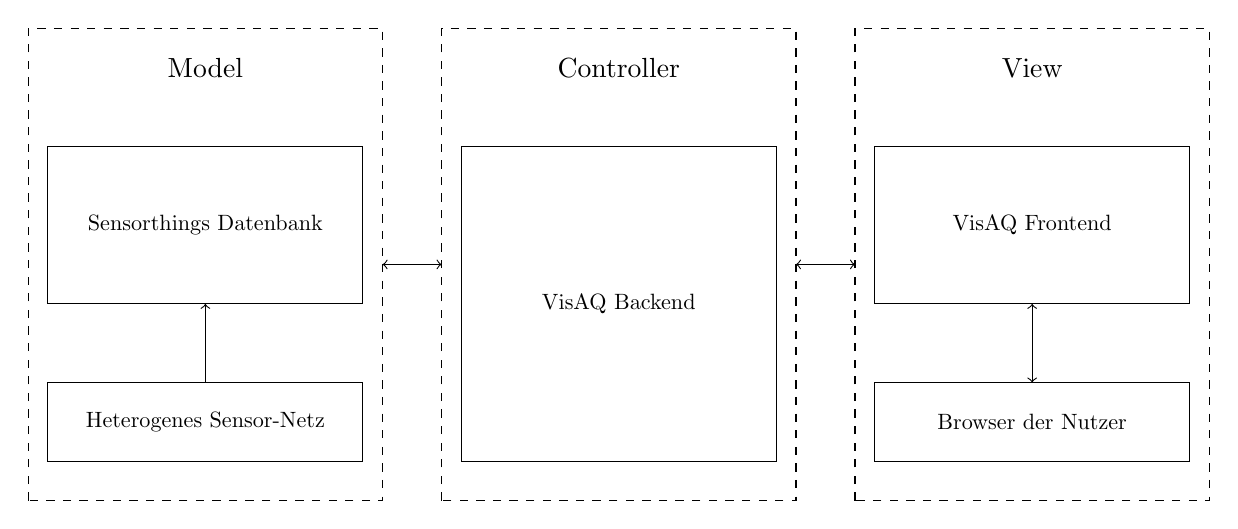
\begin{tikzpicture}[node distance=2cm]

        %Model
        \begin{scope}[shift={(0,0)},local bounding box=M]
            \draw (0,0) [dashed] rectangle (4.5,6);
            \node[scale=1] at (2.25,5.5) {Model};
            \begin{scope}[local bounding box=Datenbank]
                \draw (0.25,2.5) rectangle (4.25,4.5);
                \node[scale=0.8] at (2.25,3.5) {Sensorthings Datenbank};
            \end{scope}
            \begin{scope}[local bounding box=Sensoren]
                \draw (0.25,0.5) rectangle (4.25,1.5);
                \node[scale=0.8] at (2.25,1) {Heterogenes Sensor-Netz};
            \end{scope}
        \end{scope}
        
        %Controller
        \begin{scope}[shift={(5.25,0)},local bounding box=C]
            \draw (0,0) [dashed] rectangle (4.5,6);
            \node[scale=1] at (2.25,5.5) {Controller};
            \begin{scope}[local bounding box=Backend]
                \draw (0.25,0.5) rectangle (4.25,4.5);
                \node[scale=0.8] at (2.25,2.5) {VisAQ Backend};
            \end{scope}
        \end{scope}

        %View
        \begin{scope}[shift={(10.5,0)},local bounding box=V]
            \draw (0,0) [dashed] rectangle (4.5,6);
            \node[scale=1] at (2.25,5.5) {View};

            \begin{scope}[local bounding box=Frontend]
                \draw (0.25,2.5) rectangle (4.25,4.5);
                \node[scale=0.8] at (2.25,3.5) {VisAQ Frontend};
            \end{scope}
            \begin{scope}[local bounding box=Browser]
                \draw (0.25,0.5) rectangle (4.25,1.5);
                \node[scale=0.8] at (2.25,1) {Browser der Nutzer};
            \end{scope}
        \end{scope}

            
        \draw[<->] (M.east) -- (C.west);
        \draw[<->] (C.east) -- (V.west);
        \draw[<-] (Datenbank.south) -- (Sensoren.north);
        \draw[<->] (Frontend.south) -- (Browser.north);

    \end{tikzpicture}
    \caption{Diagram des System-Aufbaus}
\end{figure}